%© Antoine Martinet, oct 2014. All rights reserved.
%paper, layout
\documentclass{beamer}
\usetheme{Darmstadt}
%\usetheme{Dresden}
\usecolortheme[]{default}
\setbeamercolor*{palette primary}{use=structure, fg=gray!20, bg=red!70!black}
\setbeamercolor*{palette secondary}{use=structure, fg=blue, bg=red!50!black}
%\setbeamercolor*{palette tertiary}{use=structure, fg=green, bg=green}
%\setbeamercolor{titlelike}{parent=structure, fg=lightgray, bg=red!60!black}
%\setbeamercolor{subsection in head/foot}{bg=gray!30,fg=black}
\setbeamercolor{section number projected}{bg=red!100!black,fg=black!80}
\setbeamercolor{subsection number projected}{bg=red!100!black,fg=black!80}
\setbeamercolor{subsubsection number projected}{bg=red!100!black,fg=black!80}

%\usetheme{Marburg}
\usepackage[utf8]{inputenc}

\usepackage{multicol}

\usepackage{bibentry}
\nobibliography*

%images, pdf pages inclusions
\usepackage{pdfpages}
\usepackage{pgfpages}

%hypertext links
\usepackage{hyperref}
\hypersetup{
	colorlinks=true,
	breaklinks=true,
	linkcolor=black!45,
	urlcolor=blue}

%graphics and handmade figures
\usepackage{graphicx}
\usepackage{tikz}
\usetikzlibrary{arrows,shapes}
\usetikzlibrary{calc}
\newcommand{\msbout}{m_{\text{out}}}
\newcommand{\appr}[1]{\widetilde{#1}}
\newcommand{\yout}{y_{\text{out}}}
\newcommand{\abserr}{\varepsilon}
\newcommand{\epssopc}{\abserr_{\text{r}}}
\newcommand{\epsfinalround}{\abserr_{\text{f}}}
\newcommand{\TODO}{\textbf{TODO}}
\tikzset{
  x=1ex,y=1ex,
  hwblock/.style={draw, rectangle, rounded corners=.3, very thick, fill=black!5, font=\sf, minimum height=5ex},
  hwbus/.style={very thick,>=stealth},
  hwwire/.style={thin, >=stealth, },
  hwword/.style={draw, rectangle, minimum height=3ex},
  bitwidth/.style={font=\scriptsize,midway,right}
}

%slide number on the left of the footer
 \setbeamertemplate
  {footline}{\hspace{5pt}\insertframenumber/\inserttotalframenumber\strut\quad\hfill\vspace{3pt}} 

\title{Architecture Synthesis \\ for \\ Linear Time-Invariant Filters}
%\author{\\ \Large Antoine Martinet \\ \\\\\\\\\\\\\\ \\ \\ Master 2 Internship Report \\ \\ \\ \LARGE at CITI lab \\ INRIA's SOCRATE Team \\\\\\\\\\\\\\\\ \normalsize under the supervision of\\ \\ \Large Florent de Dinechin \\ \\ \\}
%\date{2 February - 31 Jully, \\ \vspace{5pt} 2015}

\author[author]{Antoine Martinet}
\date{2 February - 31 July, \vspace{5pt} 2015}
\institute{CITI lab, \\ INRIA's SOCRATE Team, \\ \vspace{5pt} Under the supervision of \\Florent de Dinechin}

%\AtBeginSection[]
%{
%	\begin{frame}
%	\transdissolve
%		\frametitle{Table of Contents}
%		\tableofcontents[currentsection]
%	\end{frame}
%}
%\AtBeginSubsection[]
%{
%	\begin{frame}
%	\transdissolve
%		\frametitle{Table of Contents}
%		\tableofcontents[currentsection,currentsubsection]
%	\end{frame}
%}

\usepackage{xspace}
\usepackage{array}
\usepackage{tabularx}

%\usepackage{stmaryrd}
\usepackage[]{algorithm2e}
\usepackage{amssymb}
%\usepackage[?]{amsmath}
\usepackage{epsfig}
\usepackage{enumerate}
\usepackage{comment}
\setcounter{MaxMatrixCols}{20}

\usepackage[]{xcolor}
\definecolor{light-gray}{gray}{0.6}
\definecolor{blue}{RGB}{0,0,153}
\definecolor{blue1}{RGB}{0,102,204}
\definecolor{blue2}{RGB}{51,153,255}
\definecolor{blue3}{RGB}{0,153,153}
\definecolor{blue4}{RGB}{102,102,255}
\definecolor{red1}{RGB}{255,0,0}
\definecolor{orange1}{RGB}{255,153,51}
\definecolor{green}{RGB}{0,204,0}
\definecolor{purple}{RGB}{204,0,204}

\begin{document}

	\begin{frame}
	\maketitle
	\end{frame}

	\begin{frame}
	\tableofcontents
	\end{frame}

	\section{Introduction}
	\begin{frame}
		\frametitle{Introduction}

	\end{frame}

	
	\section{Signal processing and filters}
		\subsection[Fundamentals about signal processing]{Fundamentals about signal processsing\footnote{For a more complete introduction to the domain, please see appendix \ref{norem}} }
	\subsubsection{Definition of a signal}
	Lopez's PhD \cite{lopez} gives a good presentation of the state of the art.
	Many notations and definitions are kept from this PhD.

	Note that a bold symbol (for example $\boldsymbol{h}$) denotes a matrix, that may be a vector.
	On the contrary, a normal symbol (for example $\varepsilon_{t_1}(k)$) denotes a single value

	\begin{thdef}\label{sig} (Signal)
		Generally, a signal is a temporal variable, which takes a value from $\mathbb{R}$ at each time t.
		$x(t)$ denotes the value of the signal $x$ at the instant $t$.
		When dealing with discrete time events, the time will be represented by $k$.
		The notation will then be $x(k)$, which is said to be a sample.
		$\{x(k)\}_{k \geq 0}$ denotes all the values possible for the signal x.
		The rest of this report adresses vectors of signals $\textbf{x}$, where $\textbf{x}(k) \in \mathbb{R}^{n}$
	\end{thdef}

	%\subsubsection{$l^\infty$ norm}
	%\begin{thdef}\label{l_inf} ($\ell^\infty$ norm)
	%	The $\ell^\infty$ norm of a scalar signal x, denoted $\|x\|_{\ell^\infty}$, is the smallest upper bound among all values (absolute values) possible for the signal x, that is:
	%	\begin{equation} \label{l3}
	%			\|x\|_{\ell^\infty}=\sup_{k\in \mathbb{N}}|x(k)|
	%	\end{equation}
	%\end{thdef}

	\subsubsection[Linear Time Invariant Filters (LTI Filters)]{Linear Time Invariant Filters (LTI filters)\footnote{For more information about the studied filters, please refer to appendix \ref{fildef}}}
	A filter, denoted by its transfer function $\mathcal{H}$, is an application which transforms a signal vector $\boldsymbol{u}$ (with $dim(\boldsymbol{u}) = n_u$ )
	into a signal vector $\boldsymbol{y} = \mathcal{H}(\boldsymbol{u})$, of size $dim(\boldsymbol{y}) = n_y$ . The case where $n_u = n_y = 1$ is referred as Single Input Single Output
	(SISO) filters. Other cases are referred as Multiple Input Multiple Output (MIMO) filters.

	\begin{thdef} (Linear Time Invariant Filter)

		Linearity:
		$$ \mathcal{H}(\alpha \cdot \boldsymbol{u}_1+ \beta \cdot \boldsymbol{u}_2)= \alpha\cdot\mathcal{H}(\boldsymbol{u}_1) +  \beta\cdot\mathcal{H}(\boldsymbol{u}_2)$$

		Time invariance:
		$$ \{\mathcal{H}(\boldsymbol{u})(k-k_0)\}_{k\geq0} = \mathcal{H}(\{\boldsymbol{u}(k-k_0)\}_{k \geq 0} ) $$
	\end{thdef}

	%\subsubsection{Impulse response}
	%\begin{thdef} (Impulse Response)
	%A SISO filter may be defined by its impulse response, denoted $h$. $h$ is the
	%impulse response of H to the impulsion of Dirac.
	%Indeed each input signal can be described as a sum of Dirac impulsions:
	%$$u=\sum_{i\geq0}u(l)\delta_l$$
	%where $\delta_l$ is a Dirac impulsion centered in $l$, that is:
	%\begin{equation}
	%	\delta_l(k) =
	%	\begin{cases}
	%		1 & \hspace{5pt} when \hspace{5pt} k=l\\
	%		0 & \hspace{5pt} else\\
	%	\end{cases}
	%\end{equation}
	%The linearity condition of $\mathcal{H}$ implies: $\mathcal{H}(u) = \sum_{l\geq0}u(l)\mathcal{H}(\delta_l)$.
	%Time invariance gives: $\mathcal{H}(\delta_l)(k)=h(k-l)$.
	%Then the computation from inputs to outputs takes this form:
	%$$y(k)=\sum_{l\geq0}u(l)h(k-l)=\sum_{l=0}^ku(k)h(k-l)$$
	%This corresponds with the convolution product definition of $u$ by $h$, denoted $y = h * u$.
	%%Dealing with MIMO filters, we have $\boldsymbol{h} \in \mathbb{R}^{n_y \times n_u}$ as the impulse response of $\mathcal{H}$. $\boldsymbol{h}_{i,j}$ is the response on the
	%Dealing with MIMO filters, $\boldsymbol{h}(k) \in \mathbb{R}^{n_y \times n_u}$ is the impulse response of $\mathcal{H}$. $\boldsymbol{h}_{i,j}(k)$ is the response on the
	%ith output to the Dirac implusion on the j-th input.
	%The precedent equation becomes:
	%$$y_i(k)=\sum_{j=1}^{n_u}\sum_{l=0}^ku_j(l)h_{i,j}(k-l), \hspace{5pt} \forall 1 \leq i \leq n_y$$
	%
	%\end{thdef} 

	\subsubsection{Worst-Case Peak Gain (WCPG) of a Filter: the maximum possible amplification}
	\begin{thdef} (Worst-Case Peak Gain)
		The worst case peak gain is defined as the maximum amplification
		possible over all potential inputs through the filter.
		$$\|\mathcal{H}\|_{wcpg}=\sup_{u\neq0}\frac{\|h*u\|_{l^{\infty}}}{\|u\|_{l^{\infty}}}$$
		with $h$ the impulse response of $\mathcal{H}$, $u$ the input signal, and $h * u$ the convolution product of $h$ by $u$ (output of the
				filter).
	
	\end{thdef}
%	\subsection{FIR and IIR: two filters families}
%	There are two types of LTI filters: \textit{Finite impulse response} (FIR) and \textit{Infinite impulse response} (IIR) filters.
%	Formally, the impulse response is finite when:
%	\begin{equation} \label{finimp}
%		\exists n \in \mathbb{N} | \forall k \geq n, h(k)=0
%	\end{equation}
%	The smallest $n$ verifying \ref{finimp} is referred as the order of the filter. So a $n$-order FIR can be described by the
%	following equation:
%	\begin{equation} \label{firdef}
%		y(k)=\sum_{i=0}^n b_i u(k-i)
%	\end{equation}
%
%	An IIR will be described as following:
%	\begin{equation} \label{iirdef}
%		y(k)=\sum_{i=0}^n b_i u(k-i) - \sum_{i=0}^n a_i y(k-i)
%	\end{equation}
%
%	%Here one can observe that the output at time $k$ depends also on all previous $n$ outputs (loopback). 
%	%Also remark that a FIR can be seen as an IIR with $\forall i \in [0,n],a_i=0$
%	%The impulse response can then be deduced from \ref{iirdef} by resolving the recurrence relation:
%
%	%\begin{equation}
%	%	h(k) =
%	%	\begin{cases}
%	%		0 & when \hspace{5pt} k<l\\
%	%		b_k - \sum_{l=1}^n a_l h(k-l) & when \hspace{5pt} 0\leq k \leq n\\
%	%		\sum_{l=1}^n a_l h(k-l) & when \hspace{5pt} n< k\\
%	%	\end{cases}
%	%\end{equation}

	\subsection{Different realizations: how to compute the output of a filter?}
	\begin{thdef} (realization)
	A realization can be defined as an algorithm describing how to compute outputs
	from inputs. However, a realization does not describes the details of basic operations (format, size,
	rounding, etc...)
	\end{thdef}
	It is important to know that all realizations of a filter are mathematically equivalent to each other (infinite
	precision). But in finite precision, rounding aspects have a huge impact on the correctness of results.
	Most of the time in this report, realizations will be referred as forms.

%	\subsubsection{Direct and transposed forms}
%	Direct and transposed forms are classic realizations. A good description of these forms can be found in Lopez’ and Hilaire’s PhDs \cite{lopez} \cite{hilaire}. 
%	The direct form has been implemented in the FoPoCo project,
%	The hardware implementation of anIIR can be seen on figure \ref{fig:ltiarch}
%
%\begin{figure*}[h]
%  \centering
%  \begin{tikzpicture}
%     \draw[dotted,black, fill=yellow!20] (-5ex,-3.5ex) rectangle +(69ex,-15ex);   
%     \node[black]  at (-2ex,-17.5ex) {{\small SOPC}};   
%    \draw[hwbus] (-8, 0) node[left] {$u(k)$} --  ++(8, 0)  ;
%    \draw[hwbus,->] (-8, 0) --  ++(3, 0); % just for the arrow
%    \foreach \i in {0,...,3} {
%      \draw[hwbus, ->] ($(8*\i, 0)$) --  ++(0, -5);
%      \draw[hwblock] ($(8*\i, -5)$) -- ++(3, 0) -- ++(-3, -4) -- ++(-3, 4) -- cycle; 
%      \node (n) at ($(8*\i , -6.5)$)  {$b_{\i}$} ;
%%      \draw ($(8*\i  + 0.5, -11)$) node[left,tt=black!50] {\footnotesize $p_b(k,\i)$} ;
%%      \draw ($(8*\i  - 0.2, -11)$) node[right,text=black!50] {\footnotesize $p_b(k,\i)$} ;
%
%%      \draw[hwbus, ->] ($(8*\i ex, 0ex)$) --  ++(0, -5ex);
%    }
%
%    
%    \draw[hwbus] (0, -9) -- ++(0,-6);
%      \coordinate (n) at  (0,-15);
%    \foreach \i in {1,...,3} {
%      \draw[line width=3pt] ($(8*\i  - 4, -3)$) --  +(0, 6);
%      \draw[hwbus] ($(8*\i  - 8, 0)$) --  +(8,0) node [above,text=blue] {\footnotesize $u(k-\i)$};
%      \draw[hwbus,->] ($(8*\i  - 8, 0)$) --  ++(3, 0); % just for the arrow
%      % The adders 
%      \coordinate (nm1) at  (n.east);
%      \draw ($(8*\i , -15)$) node[hwblock,circle,minimum height=3] (n) {$+$};
%      \draw[hwbus, ->]  ($(8*\i , -9)$) -- (n.north);
%      \draw[hwbus, ->]  (nm1) -- (n.west);
%      \draw[hwbus]  (n.east) -- ++ (3,0);
%    }
%
%    \draw (74, -15) node[hwblock,align=center] (fr) {final\\round} ;
%    \draw[hwbus, <-] (fr.west) -- ++(-15,0) node [near end] {/} node [near end,below] {\footnotesize$(\msbout, p-g$)} node[near start,above] {$\appr{y}(k)$} -- ++(-1,0) ;
%    \draw[hwbus, ->] (fr.east) -- ++(8,0) node [midway] {/} node [midway,below] {\footnotesize$(\msbout,p)$} node[right] {$\yout(k)$} ;
%
%    \foreach \i in {1,...,3} {
%      \draw[hwbus, ->] ($(-8*\i  + 60 , 0)$) --  ++(0, -5);
%      \draw[hwblock] ($(-8*\i  + 60 , -5)$) -- ++(3, 0) -- ++(-3, -4) -- ++(-3, 4) -- cycle; 
%      \node (ai) at ($(-8*\i  + 60 , -6.5)$)  {$a_{\i}$} ;
%      %\draw ($(-8*\i  +60 + 0.5, -11)$) node[left,text=black!50] {\footnotesize $p_a(k,\i)$} ;
%      %\draw ($(-8*\i  +60 - 0.2, -11)$) node[right,text=black!50] {\footnotesize $p_a(k,\i)$} ;
%      \draw ($(-8*\i  + 60 , -15)$) node[hwblock,circle,minimum height=3] (n) {$+$};
%      \draw (n.north) node[left]{\bf -};
%      \draw[hwbus, ->] ($(-8*\i  + 60, -9)$) --  (n.north);
%      \draw[hwbus, <-] (n.west) -- ++(-5,0);
%      % The registers
%      \draw[hwbus] ($(-8*\i  + 60  +8, 0)$) --  ++(-8, 0) node [above,text=blue] {\footnotesize $\appr{y}(k-\i)$};
%      \draw[hwbus,->] ($(-8*\i  + 60  +8, 0)$) --  ++(-3, 0); % just for the arrow
%      \draw[line width=3pt] ($(-8*\i  +60 + 4, -3)$) --  +(0, 6);
%    }
%    \draw[hwbus] ($(60 , 0)$) --  ++(0,-15);
%    \draw[hwbus,<-] ($(60 , -5)$) --  ++(0,-5);
%
%
%  \end{tikzpicture}
%
%\caption{Abstract architecture for the direct form realization of an LTI filter \label{fig:ltiarch}}
%\end{figure*}
%
%	\subsubsection{State-space representation: a recurrence to define an infinite response}
	%This type of realization consists in expressing the evolution of a system considering its state at time $k$. In
	\vspace{10pt}
	The state-space representation is a type of realization consists in expressing the evolution of a system considering its state at time $k$. In
	continuous time, it is described by differential equations at first order. In discret time (in which we
	are interested in), it is described by a simple recurrence:
	\begin{equation} \label{abcddef}
		\begin{cases}
			\boldsymbol{x}(k+1)= \boldsymbol{Ax}(k) + \boldsymbol{Bu}(k) \\
			\boldsymbol{y}(k+1)= \boldsymbol{Cx}(k) + \boldsymbol{Du}(k)
		\end{cases}
	\end{equation}

	Where $\boldsymbol{x}(k) \in \mathbb{R}^{n_x}$ is the state vector,
	$\boldsymbol{u}(k) \in \mathbb{R}^{n_u}$ is the input vector and
	$\boldsymbol{y}(k) \in \mathbb{R}^{n_y}$ is the output vector, at time k.
	The matrices $\boldsymbol{A} \in \mathbb{R}^{n_x \times n_x}$ , $\boldsymbol{B} \in \mathbb{R}^{n_x \times n_u}$,
	$\boldsymbol{C} \in \mathbb{R}^{n_y \times n_x}$, and $\boldsymbol{D} \in \mathbb{R}^{n_y \times n_u}$,
	with $\boldsymbol{x}(0)$ are sufficient to describe an LTI filter, with convention $\boldsymbol{x}(k)=\boldsymbol{u}(k)=0 \hspace{5pt}, \hspace{5pt} \forall k<0$.

	\subsection{The Specialized Implicit Form (SIF): a unified representation}
	\subsubsection{Definition}
	The classical state-space representation is intuitive, but it doesn't take into account the reality of implementation.
	The specialized implicit form (SIF) was introduced in \cite{sifd}, is well detailed in Hilaire's PhD and associated papers \cite{hilaire,sif},
	and is a good answer to this problem.
	Indeed, dealing with finite precision and error amplification, the order in which operations are done becomes crucial.
	Another motivation is to have a unique representation for any realization of LTI filters,
	that allows to compute every degradation measures instead of redevelopping them for each new realization.
	This form distinguishes computations done at one time from computations done the other times. As well as
	in a state-space, $\boldsymbol{x}$-coordinates are state variables, but in addition to that, $\boldsymbol{t}$-coordinates are intermediate variables.
	The SIF is described as following:
	\begin{equation} \label{sifdef}
		\begin{pmatrix}
			\boldsymbol{J} & \boldsymbol{0} & \boldsymbol{0} \\
			\boldsymbol{-K} & \boldsymbol{I}_{n_x} & \boldsymbol{0} \\
			\boldsymbol{-L} & \boldsymbol{0} & \boldsymbol{I}_{n_y} 
		\end{pmatrix}
		\begin{pmatrix}
			\boldsymbol{t} (k+1)  \\
			\boldsymbol{x} (k+1)  \\
			\boldsymbol{y} (k) 
		\end{pmatrix}
		=
		\begin{pmatrix}
			\boldsymbol{0} & \boldsymbol{M} & \boldsymbol{N} \\
			\boldsymbol{0} & \boldsymbol{P} & \boldsymbol{Q} \\
			\boldsymbol{0} & \boldsymbol{R} & \boldsymbol{S} 
		\end{pmatrix}
		\begin{pmatrix}
			\boldsymbol{t} (k)  \\
			\boldsymbol{x} (k)  \\
			\boldsymbol{u} (k) 
		\end{pmatrix}
	\end{equation}
%	With $n_t$, $n_x$, $n_y$ and $n_u$ the sizes of $\boldsymbol{t}$, $\boldsymbol{x}$, $\boldsymbol{y}$ and $\boldsymbol{u}$, respectively.
%	$\boldsymbol{J}$, is a lower triangular matrix, with
%	diagonal entries equal to 1.
%	%Then we have the following dimensions for the previous matrices:
%	The previous matrices have the following dimensions:
%
%	\begin{eqnarray}
%		\boldsymbol{J} \in \mathbb{R}^{n_t \times n_t},\boldsymbol{M} \in \mathbb{R}^{n_t \times n_x},\boldsymbol{N} \in \mathbb{R}^{n_t \times n_u}, \nonumber \\
%		\boldsymbol{K} \in \mathbb{R}^{n_x \times n_t},\boldsymbol{P} \in \mathbb{R}^{n_x \times n_x},\boldsymbol{Q} \in \mathbb{R}^{n_x \times n_u}, \\
%		\boldsymbol{L} \in \mathbb{R}^{n_y \times n_t},\boldsymbol{R} \in \mathbb{R}^{n_y \times n_x},\boldsymbol{S} \in \mathbb{R}^{n_y \times n_u}, \nonumber \\
%	\end{eqnarray}

	The best way to understand the SIF may be to see it as an algorithm, each line of the equation \ref{sifdef} corresponding to a sequential step of the computation.
	%The algorithm results as follows:
	%\begin{algorithm}
	%	\For{int i = 0 ; $i \leq n_t$; i++}{
	%		$\boldsymbol{t}_i(k+1) \leftarrow - \sum\limits\limits_{j<i} \boldsymbol{J}_{ij}\boldsymbol{t}_j(k+1) + \sum\limits_{j=1}^{n_x} \boldsymbol{M}_{ij}\boldsymbol{x}_j(k) + \sum\limits_{j=1}^{n_u} \boldsymbol{N}_{ij}\boldsymbol{u}_j(k)$
	%	}
	%	\For{int i = 0 ; $i \leq n_x$; i++}{
	%		$\boldsymbol{x}_i(k+1) \leftarrow - \sum\limits_{j=1}^{n_t} \boldsymbol{K}_{ij}\boldsymbol{t}_j(k+1) + \sum\limits_{j=1}^{n_x} \boldsymbol{P}_{ij}\boldsymbol{x}_j(k) + \sum\limits_{j=1}^{n_u} \boldsymbol{Q}_{ij}\boldsymbol{u}_j(k)$
	%	}
	%	\For{int i = 0 ; $i \leq ny$; i++}{
	%		$\boldsymbol{y}_i(k) \leftarrow - \sum\limits_{j=1}^{n_t} \boldsymbol{L}_{ij}\boldsymbol{t}_j(k+1) + \sum\limits_{j=1}^{n_x} \boldsymbol{R}_{ij}\boldsymbol{x}_j(k) + \sum\limits_{j=1}^{n_u} \boldsymbol{S}_{ij}\boldsymbol{u}_j(k)$
	%	}
	%	\caption{Computation of SIF outputs from inputs}
	%\end{algorithm}

	%Here, it is important to see that the form of $\boldsymbol{J}$ allows to compute the $\boldsymbol{t}_i$ sequentially. The algorithm can
	%then be described as follows:
	%\begin{algorithm} \label{algomat}
	%	\For{int i = 0 ; $i \leq n_t$; i++}{
	%		$\boldsymbol{t}_i(k+1) \leftarrow - \boldsymbol{J'}_{i}\boldsymbol{t}(k+1) + \boldsymbol{M}_{i}\boldsymbol{x}(k) +\boldsymbol{N}_{i}\boldsymbol{u}(k)$
	%	}
	%	\For{int i = 0 ; $i \leq n_x$; i++}{
	%		$\boldsymbol{x}_i(k+1) \leftarrow - \boldsymbol{K}_{i}\boldsymbol{t}(k+1) + \boldsymbol{P}_{i}\boldsymbol{x}(k) +\boldsymbol{Q}_{i}\boldsymbol{u}(k)$
	%	}
	%	\For{int i = 0 ; $i \leq ny$; i++}{
	%		$\boldsymbol{y}_i(k) \leftarrow - \boldsymbol{L}_{i}\boldsymbol{t}(k+1) + \boldsymbol{R}_{i}\boldsymbol{x}(k) + \boldsymbol{S}_{i}\boldsymbol{u}(k)$
	%	}
	%	\caption{Simplified matricial algorithm}
	%\end{algorithm}

	%With $\boldsymbol{J'} = \boldsymbol{J} - I_{n_t}$.

	Values of the vector $\boldsymbol{t}(k+1)$ are computed and used at the same iterations, so they are not kept in memory.
	As the equation \ref{sifdef} is mostly full of zeros, it is more convenient to use it’s compressed formulation, which is denoted
	$\boldsymbol{Z}$:
	
	\begin{equation} \label{zmatrix}
		\boldsymbol{Z}=
		\begin{pmatrix}
			\boldsymbol{-J} & \boldsymbol{M} & \boldsymbol{N} \\
			\boldsymbol{K} & \boldsymbol{P} & \boldsymbol{Q} \\
			\boldsymbol{L} & \boldsymbol{R} & \boldsymbol{S} 
		\end{pmatrix}
	\end{equation}

	The community usually takes $-\boldsymbol{J}$ for simplicity within further computations.

	%The SIF can of course be transformed into an equivalent ABCD (classic state-space) form, which gives:
	The SIF can of course be transformed into an equivalent ABCD (classic state-space) form.
	About parallelism, it is useful to remark that $t(k+1)$ are computed sequentially, while $x(k+1)$ and $y(k)$ can be computed in parallel.
%
%	\begin{eqnarray} \label{abcdtranspose}
%		\boldsymbol{A_Z} = \boldsymbol{KJ}^{-1}\boldsymbol{M} +\boldsymbol{P}, \hspace{5pt}
%		\boldsymbol{B_Z} = \boldsymbol{KJ}^{-1}\boldsymbol{N} +\boldsymbol{Q}, \nonumber \\
%		\boldsymbol{C_Z} = \boldsymbol{LJ}^{-1}\boldsymbol{M} +\boldsymbol{R}, \hspace{5pt}
%		\boldsymbol{D_Z} = \boldsymbol{LJ}^{-1}\boldsymbol{N} +\boldsymbol{S}, \nonumber \\
%	\end{eqnarray}
%
%	with:
%	\begin{eqnarray}
%		\boldsymbol{A_Z} \in \mathbb{R}^{n_x \times n_x},
%		\boldsymbol{B_Z} \in \mathbb{R}^{n_x \times n_u}, \nonumber \\
%		\boldsymbol{C_Z} \in \mathbb{R}^{n_y \times n_x},
%		\boldsymbol{D_Z} \in \mathbb{R}^{n_y \times n_u},
%	\end{eqnarray}

	\subsubsection{Workflow for filter implementation}
		%Here, we won't discuss the optimality of the SIF description.
		The choice of the SIF realization is not concerned by this work.
		This choice is up to the user, who may have a lot of good reasons not to design a realization that seem intuitive for us.
		The choice of the realization is a job done at LIP6 in the PEQUAN team, under the metalibm ANR project.
		The present work is just a hardware backend for the choice part.
		Of course, optimizations are available at every level.
		The expected use of this work is shown on figure \ref{fig:workflow}.


		\begin{figure}[h] 
		  \centering
		  \begin{tikzpicture}[x=0.8cm,y=1cm]
			\draw (-9.5, 1.0) -- (-8,1.0) [->, thick] node[above,near start, text width = 3cm, align=center]{User filter specification};
			\draw (-3.5, 1.0) -- (0.0,1.0) [->, thick] node[below,xshift=-1.4cm]{$\begin{pmatrix}\boldsymbol{-J} & \boldsymbol{M} & \boldsymbol{M}_t \\ \boldsymbol{K} & \boldsymbol{P} & \boldsymbol{M}_x \\ \boldsymbol{L} & \boldsymbol{R} & \boldsymbol{M}_y \end{pmatrix}$};
			\draw (-8,-0.3) rectangle ++(4.5,2.4)[thick] node [midway, text width = 4cm, align=center]{Realization Choice \\ by \\ Hilaire, Volkova  \\ team PEQUAN, LIP6 \\(Front-End)}; 
			\draw (0.0,0.0) rectangle ++(3.0,2)[thick] node [midway, text width = 3cm, align=center]{Flopoco core generation \\ (this work) \\(Back-End)}; 

			\draw (4,0) rectangle ++(2.5,2)[thick] node [midway]{VHDL}; 
			\draw (3.0, 1) -- (4,1) [->, thick] node[above,near start]{};

		  \end{tikzpicture}

		\caption{Workflow overview of tools usage \label{fig:workflow}}
		\end{figure}










%	\subsection{Adjustments in arbitrary precision}

	





%		
%	\subsection{Canonical specification}
%		
%		The intuitive and first way to describe an LTI filter is to specify the output as a function of the inputs:
%		$$y(k)=\sum_{i=0}^n b_i u(k-i)-\sum_{i=1}^n a_i y(k-i)$$
%
%	\subsection{Z transform}
%	$$X(z)=\mathcal{Z}\{x\}=\sum_{k=0}^{+\infty} x(k) z^{-k}$$
%	
%	\subsection{Transfert Function}
%	A filter is usually described by it's transfert function, defined as:
%
%	$$H(z)=\frac{Y(z)}{U(z)}=\frac{\sum_{i=0}^n b_i z^{-i}}{ 1 + \sum_{i=1}^n a_i z^{-i}}, \;\;\;\; \forall z \in \mathbb{C}$$ 
%	\subsection{Impulse response}
%	$\delta$
%	\subsection{Worst case peak gain (WCPG)}
%	$$\| \mathcal{H} \|_{WCPG}=\sup_{i\neq 0} \frac{\|h*u\|_{l^\infty}}{\|u\|_{l^\infty}} $$
%
%	$$\| \mathcal{H} \|_{WCPG}= \sum_{k \geq 0} |h(k)| $$
%	\subsection{Realisations}



	





	\section{Implementation}
		\subsection{Implementation: what can be done in practise?}

	\subsubsection{The FloPoCo Framework: computing just right}
		FloPoCo is a C++ framework \cite{DinechinPasca2011-DaT} which first purpose is to generate floating point cores in VHDL.
		It targets the configuration of FPGAs as computing units, and could also be useful dealing with ASIC specification.
		Indeed, FPGAs are well used for embedded computing, because they offer full reconfigurability and a relatively good balance between computation power and price.

		More information is available at \url{http://flopoco.gforge.inria.fr/}

	This work proposes to implement SIFs using the SOPC arithmetical core from FloPoCo.
	SOPC stands for Sum of Products by Constants, and is a KCM-multiplier based architecture.
	The details of the SOPC architecture has been described in \cite{sums}.

	\subsubsection{KCM multipliers: an architecture to efficiently compute products on FPGAs}
	To be quick, a KCM multiplier is designed to fully use the power of look-up tables (LUTs) of an FPGA.
	To do so, it partitions the constant into chunks which match the size of a LUT.
	Then, tabulating the multiplications ends up with a final sum to compute the product.
	This has been first described by K.Chapman in \cite{Chapman93:edn}.
	The detail of implementation is visible on figure \ref{fig:FixRealKCM}

\begin{figure}[b]
  \begin{center}
  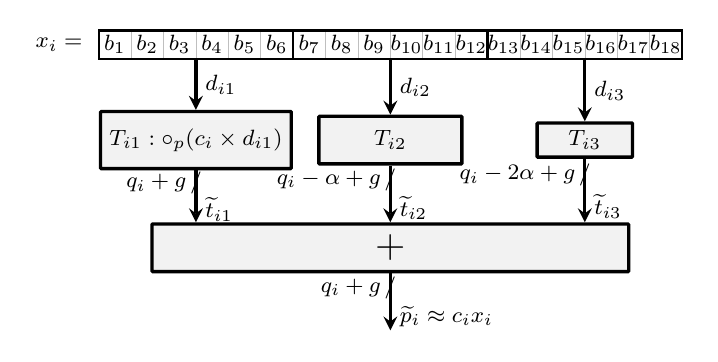
\begin{tikzpicture}
    \footnotesize 
    \node at (-1em,0)  {$x_i=$} ;
    \foreach \x in {1,...,18} {
%    \draw[] ($(-5*\x ex, -7ex)$) -- ($(-5*\x ex, -5ex)$) node[above] {$2^\x$} ;
      \node (n) at ($(3.4*\x ex, 0ex)$)  {$b_{\x}$} ;
      \draw[black!25, very thin] ($(n)+(1.7ex,1.5ex)$) -- ++(0, -3ex);
    }
    \node[draw, thick, rectangle, minimum width = 3.4*6ex, minimum height=3ex] (d1) at (3.4*3ex+1.7ex,0) {} ;
    \node[hwblock, minimum width=20ex,minimum height=6ex] (T1) at ($(d1)+(0,-10ex)$) { $T_{i1}: \circ_p(c_i\times d_{i1})$};
    \draw[hwbus,->] (d1.south) --  (T1.north) node[midway,right] {$d_{i1}$};

    \node[draw, thick, rectangle, minimum width = 3.4*6ex, minimum height=3ex] (d2) at (3.4*9ex+1.7ex,0) {} ;
    \node[hwblock, minimum width=15ex] (T2) at ($(d2)+(0,-10ex)$) { $T_{i2}$};
    \draw[hwbus,->] (d2.south) --  (T2.north) node[midway,right] {$d_{i2}$};

    \node[draw, thick, rectangle, minimum width = 3.4*6ex, minimum height=3ex] (d3) at (3.4*15ex+1.7ex,0) {} ;
    \node[hwblock, minimum width=10ex,minimum height=3.5ex] (T3) at ($(d3)+(0,-10ex)$) { $T_{i3}$};
    \draw[hwbus,->] (d3.south) --  (T3.north) node[midway,right] {$d_{i3}$};

    
    \node[hwblock, minimum width=50ex] (sum) at ($(T2)+(0,-11.3ex)$) {\Large $+$};
    \draw[hwbus,->]  (T1.south) --  ($(sum.80)!(T1)!(sum.north)$) % This means: point that is the projection of T1 on the line  (sum.80) -- (sum.north)
       node[near start] {$/$} node[near start,left] {$q_i+g$}          node[near end,right] {$\widetilde{t}_{i1}$};
    \draw[hwbus,->]  (T2.south) --  ($(sum.80)!(T2)!(sum.north)$) node[near start] {$/$} node[near start,left] {$q_i-\alpha+g$}   node[near end,right] {$\widetilde{t}_{i2}$};
    \draw[hwbus,->]  (T3.south) -- ($(sum.80)!(T3)!(sum.north)$) node[near start] {$/$} node[near start,left] {$q_i-2\alpha+g$}  node[near end,right] {$\widetilde{t}_{i3}$};

    \draw[hwbus,->] (sum.south) --  ++(0,-6ex) node[near start] {$/$} node[near start,left] {$q_i+g$} node[near end,right] {$\widetilde{p}_i\approx c_ix_i$};
 \end{tikzpicture}
\end{center}
\caption{The FixRealKCM method when $x_i$ is split in 3 chunks   \label{fig:FixRealKCM}}
\end{figure}

	\subsubsection{SOPCs: exploiting full parallel architecures}

	The SOPC architecture keeps the same idea.
	%The difference is, the summation architecture is mutualized through the $n_c$ products in a bit-heap based architecture implemented by flopoco.
	The difference resides in the mutualization of the summation architecture through the $n_c$ products.
	This summation is performed within a bit-heap based architecture implemented by FloPoCo.
	The detail is visible on figure \ref{fig:Overall architecture}.

	To generate such cores, FloPoCo needs a number format specification, that is, the most significant bit (msb) and last significant bit (lsb) for the inputs and output of each operator to generate.

\begin{figure}
  \begin{center}
  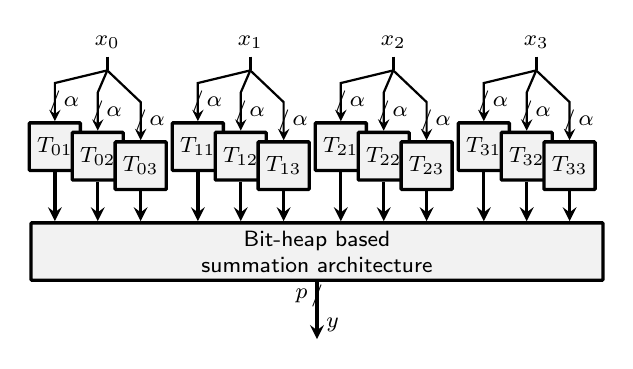
\begin{tikzpicture}
    \footnotesize 
    
    \node[hwblock, align=center,minimum width=60ex] (sum) at ($(32ex,-5ex)$) {Bit-heap based \\ summation architecture};

    \foreach \i in {0,...,3} {
      \node (x) at  ($(15*\i ex+10ex, 17ex)$) {$x_\i$};
      \coordinate (xb) at  ($(x)+(0, -3ex)$);
      \draw[hwbus,very thick] (x) --  (xb);
      
      \foreach \k in {1,...,3} {
        \node[hwblock, minimum width=5ex] (T) at ($(15*\i ex+4.5*\k ex,7ex-1*\k ex)$) { $T_{\i\k}$};
        \draw[hwbus,thick,<-]  (T.north) -- ++(0,+4ex) node [midway] {/}node [midway,right] {$\alpha$} -- (xb);
        \draw[hwbus,->] (T.south) --  ($(sum.north)!(T)!(sum.80)$);
      }
    }

    \draw[hwbus,->] (sum.south) --  ++(0,-6ex) node[near start] {$/$} node[near start,left] {$p$} node[near end,right] {$y$};
 \end{tikzpicture}
\end{center}
\caption{KCM-based SPOC architecture for $n_c=4$, each input being split into 3 chunks  \label{fig:Overall architecture}}
\end{figure}

	\subsubsection{Precision concerns}

	In SOPCs architectures, accuracy is deducible from the inputs/output specifications and the size of the constants.
	This is described in \cite{sums}.

	Dealing with feedback inputs to build an SOPC-based filter, the question of precision is more complicated.
	Indeed, when outputs loop back on inputs, as soon as the problem is in finite precision, the error is amplified by a certain amount, depending on the coefficients, at each pass through the filter.

	In this case the solution in the industry is to build an equivalent FIR filter by resolving the state-space recurrence.
	This leads to build an accurate hardware, but at the price of a huge waste of logic.
	The present work tries to answer this problem, trying to compute just right, keeping the recurrence and saving hardware.

	The main idea to dimension filters is to consider the total error as a single filter.
	The result of this filter is then added to the ``perfect" filter to get the final output.

%	In fixed precision, sizes are constrained to be all the same. The demonstration of the size computation has been described in Lopez' PhD \cite{lopez}.
%	The idea now is to see what and be done in arbitrary precision, trying to save a maximum of logic while keeping a right result on the precision required by the user.
	The two incoming parts are calculations from Lopez's PhD \cite{lopez}, with adaptations in the architecture context.
	Indeed, the original calculations are done for fixed precision, because they are expected to be done in software, with fixed word sizes.
	The challenge here is to produce architecture with arbitrary precision, that is, choosing the best msbs and lsbs for each basic operation.

%	Dealing with potential infinitly amplified errors, the question here seem very hard.
%	Fortunately filters considered in this work have an error amplification bounded, which allows us to use filters WCPGs.

%	Here the requirement is to compute each size at each step of the computation. Of course, the WCPG is not useful for the first part of a FIR, as it includes no loop.
%	So the WCPG is just important for the recursive part, which is the only one to introduce an infinite error amplification.

	%Direct and transposed forms are not directly transposable into SIF, but this problem is secondary.


	\subsubsection{Size computation in finite precision}
	When there are many potential realizations for a single LTI filter, the choice of one realization
	among the others is very related to the error analysis in output.
	The precision of our computations can then be defined so that the following condition is satisfied:

	\begin{equation} \label{condition}
		\varepsilon_{y_i} < 2^{-lsb_{y_i}} \hspace{5pt} \forall i \in [1,n_y]
	\end{equation}

	With $lsb_{y_i}$ the last significant bit of the output $y_i$, and $\varepsilon_{y_i}$ the error on the computation of the output $y_i$

	Following the same model, an error term for each SOPC is involved in the computation.
	All these error terms will be functions of the most significant and last significant bits (respectively msb and lsb) of every input, output and intermediate signal.
	So there is a need for computing every $\{msb_{t_i},lsb_{t_i}\}$, $\{msb_{x_i},lsb_{x_i}\}$ and $\{msb_{y_i},lsb_{y_i}\}$,

	This leads to the definition of errors introduced by the SOPCs architectures, based on the SIF computation algorithm:
		\begin{eqnarray}
				\boldsymbol{\varepsilon}_t(k) =
				- \boldsymbol{J'}\boldsymbol{t}^*(k+1) 
				+ \boldsymbol{M} \boldsymbol{x}^*(k) 
				+ \boldsymbol{N} \boldsymbol{u}(k) 
				- SOPC(\boldsymbol{J'}, \boldsymbol{M}, \boldsymbol{N}, \boldsymbol{t}^*(k), \boldsymbol{x}^*(k), \boldsymbol{u}(k)),\\
				\boldsymbol{\varepsilon}_x(k) =
				\boldsymbol{K}\boldsymbol{t}^*(k+1)
				+ \boldsymbol{P} \boldsymbol{x}^*(k)
				+ \boldsymbol{Q} \boldsymbol{u}(k)
				- SOPC(\boldsymbol{K}, \boldsymbol{P}, \boldsymbol{Q}, \boldsymbol{t}^*(k), \boldsymbol{x}^*(k), \boldsymbol{u}(k)),\\
				\boldsymbol{\varepsilon}_y(k) =
				\boldsymbol{L}\boldsymbol{t}^*(k+1)
				+ \boldsymbol{R} \boldsymbol{x}^*(k)
				+ \boldsymbol{S} \boldsymbol{u}(k)
				- SOPC(\boldsymbol{L}, \boldsymbol{R}, \boldsymbol{S}, \boldsymbol{t}^*(k), \boldsymbol{x}^*(k), \boldsymbol{u}(k)),
		\end{eqnarray}

		where
		$SOPC(\boldsymbol{L}, \boldsymbol{R}, \boldsymbol{S}, \boldsymbol{t}^*(k), \boldsymbol{x}^*(k), \boldsymbol{u}(k))$
		is the effective computation (with errors) of the sum of products.


%		\begin{eqnarray}
%				\boldsymbol{t}^*(k+1) = - \boldsymbol{J'}\boldsymbol{t}^*(k+1) + \boldsymbol{M} \boldsymbol{x}^*(k) + \boldsymbol{N} \boldsymbol{u}(k) + \boldsymbol{\varepsilon_t}(k)\\
%		\end{eqnarray}

	Let's define the following vectors:
	\begin{equation}
		\boldsymbol{\varepsilon}(k) =
		\begin{pmatrix}
			\boldsymbol{\varepsilon}_t(k) \\
			\boldsymbol{\varepsilon}_x(k) \\
			\boldsymbol{\varepsilon}_y(k) \\
		\end{pmatrix}
		=
		\begin{pmatrix}
			{\varepsilon}_{t_1}(k) \\
			{\varepsilon}_{t_2}(k) \\
			\vdots \\
			{\varepsilon}_{t_{n_t}}(k) \\
			\hspace{5pt} \\
			{\varepsilon}_{x_1}(k) \\
			{\varepsilon}_{x_2}(k) \\
			\vdots \\
			{\varepsilon}_{x_{n_x}}(k) \\
			\hspace{5pt} \\
			{\varepsilon}_{y_1}(k) \\
			{\varepsilon}_{y_2}(k) \\
			\vdots \\
			{\varepsilon}_{y_{n_y}}(k) \\
		\end{pmatrix}
	\end{equation}


		
	\subsubsection{Error analysis}

	Considering a filter $\mathcal{H}$ and it’s SIF, following
	the algorithm \ref{algomat}, in finite precision, leads to the following equations:

			\begin{eqnarray} \label{sifalgoerr}
				\boldsymbol{t}^*(k+1) = - \boldsymbol{J'}\boldsymbol{t}^*(k+1) + \boldsymbol{M} \boldsymbol{x}^*(k) + \boldsymbol{N} \boldsymbol{u}(k) + \boldsymbol{\varepsilon_t}(k)\\
				\boldsymbol{x}^*(k+1) = \boldsymbol{K}\boldsymbol{t}^*(k+1) + \boldsymbol{P} \boldsymbol{x}^*(k) + \boldsymbol{Q} \boldsymbol{u}(k) + \boldsymbol{\varepsilon_x}(k) \\
				\boldsymbol{y}^*(k) = \boldsymbol{L}\boldsymbol{t}^*(k+1) + \boldsymbol{R} \boldsymbol{x}^*(k) + \boldsymbol{S} \boldsymbol{u}(k) + \boldsymbol{\varepsilon_y}(k) 
			\end{eqnarray}
			Here $\boldsymbol{t}^*$, $\boldsymbol{x}^*$ and $\boldsymbol{y}^*$ are the computed vectors, so with computations errors.

	As $\boldsymbol{\varepsilon}$-errors come only from the SOPCs cores, another error term will symbolize the total error.
			Let's denote:
			\begin{eqnarray}
			\boldsymbol{\varepsilon}_{t_i}^*(k+1)=\boldsymbol{t}_i^*(k)-\boldsymbol{t}_i(k) \\
			\boldsymbol{\varepsilon}_{x_i}^*(k+1)=\boldsymbol{x}_i^*(k)-\boldsymbol{x}_i(k) \\
			\boldsymbol{\varepsilon}_{y_i}^*(k)=\boldsymbol{y}_i^*(k)-\boldsymbol{y}_i(k) 
			\end{eqnarray}
			the total error at instant k,
			considering computations errors and loopback, for 
			$\boldsymbol{t}$ , $\boldsymbol{x}$ and $\boldsymbol{y}$.
			The equations, corresponding to an algorithm, become:
			\begin{eqnarray} \label{deltaerr}
				\boldsymbol{\varepsilon}_t^*(k+1) = - \boldsymbol{J'}\boldsymbol{\varepsilon}_t^*(k+1) + \boldsymbol{M} \boldsymbol{\varepsilon}_x^*(k) + \boldsymbol{\varepsilon_t}(k)\\
				\boldsymbol{\varepsilon}_x^*(k+1) = \boldsymbol{K}\boldsymbol{\varepsilon}_t^*(k+1) + \boldsymbol{P} \boldsymbol{\varepsilon}_x^*(k) + \boldsymbol{\varepsilon_x}(k) \\
				\boldsymbol{\varepsilon}_y^*(k) = \boldsymbol{L}\boldsymbol{\varepsilon}_t^*(k+1) + \boldsymbol{R} \boldsymbol{\varepsilon}_x^*(k) + \boldsymbol{\varepsilon_y}(k) 
			\end{eqnarray}

			This new algorithm corresponds here to the algorithm of the SIF of a filter $\mathcal{H}_{\boldsymbol{\varepsilon}}$,
			which describes the behaviour of computation errors at time k on the output.
			The linearity condition allows to decompose the real $\mathcal{H}^*$ filter in two distinct filters:
			\begin{itemize}
				\item $\mathcal{H}$ the absolute filter in infinite precision
				\item $\mathcal{H}_{\boldsymbol{\varepsilon}}$ the error filter
			\end{itemize}

			\begin{figure}[h] 
			  \centering
			  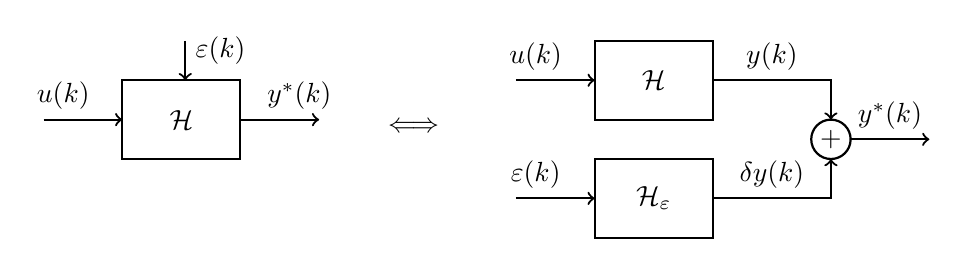
\begin{tikzpicture}[x=1cm,y=1cm]
				\draw (-9, 0.5) -- (-8,0.5) [->, thick] node[above,near start]{$\boldsymbol{u}(k)$};
				\draw (-7.2, 1.5) -- (-7.2,1.0) [->, thick] node[right,near start]{$\boldsymbol{\varepsilon}(k)$};
				\draw (-6.5, 0.5) -- (-5.5,0.5) [->, thick] node[above,near end]{$\boldsymbol{y}^*(k)$};
				\draw (-8,0.0) rectangle ++(1.5,1)[thick] node [midway]{$\mathcal{H}$}; 
				\draw (-2,0.5) rectangle ++(1.5,1)[thick] node [midway]{$\mathcal{H}$}; 
				\draw (-3, 1) -- (-2,1) [->, thick] node [above,near start]{$\boldsymbol{u}(k)$}; 
				\draw (-0.5, 1)  -- (1,1) -- (1,0.5) [->, thick] node[xshift=-0.75cm,yshift=0.8cm]{$\boldsymbol{y}(k)$}; 

				\draw (-2,-1) rectangle ++(1.5,1)[thick] node [midway]{$\mathcal{H}_{\abserr}$}; 
				\draw (-3, -0.5) -- (-2,-0.5) [->, thick] node[above,near start]{$\boldsymbol{\varepsilon}(k)$};
				\draw (-0.5, -0.5) -- (1,-0.5) -- (1,0) [->, thick] node [xshift=-0.75cm,yshift=-0.2cm]{$\boldsymbol{\delta y}(k)$}; 

				\draw (1,0.25) circle (0.25) [thick] node {$+$}; 
				\draw (1.25,0.25) -- (2.25,0.25)[->, thick] node [above,midway] {$\boldsymbol{y}^*(k)$};

				\node (arrow) at (-4.3,0.4) {$\iff$};
			  \end{tikzpicture}

			\caption{A signal view of the error propagation with respect to the ideal filter \label{fig:ltierror}}
			\end{figure}


		According to \ref{zmatrix}:

		\begin{equation} \label{zepsmatrix}
		\boldsymbol{Z_\varepsilon}=
					\begin{pmatrix}
						\boldsymbol{-J} & \boldsymbol{M} & \boldsymbol{M}_t \\
						\boldsymbol{K} & \boldsymbol{P} & \boldsymbol{M}_x \\
						\boldsymbol{L} & \boldsymbol{R} & \boldsymbol{M}_y 
					\end{pmatrix}
		\end{equation}

		with:
		\begin{eqnarray} \label{deltaerr}
			\boldsymbol{M}_t=(\boldsymbol{I}_{n_t} \hspace{5pt} \boldsymbol{0}_{n_t \times n_x} \hspace{5pt} \boldsymbol{0}_{n_t \times n_y}), \\
			\boldsymbol{M}_x=(\boldsymbol{0}_{n_x \times n_t} \hspace{5pt} \boldsymbol{I}_{n_x} \hspace{5pt} \boldsymbol{0}_{n_x \times n_y}), \\
			\boldsymbol{M}_y=(\boldsymbol{0}_{n_y \times n_t} \hspace{5pt} \boldsymbol{0}_{n_y \times n_x} \hspace{5pt} \boldsymbol{I}_{n_y}),
		\end{eqnarray}

		$\mathcal{H}_{\boldsymbol{\varepsilon}}$ is a filter with ($n_t+n_x+n_u$) inputs and $n_y$ outputs.
		\begin{proposition}
			The transfert function of filter $\mathcal{H_{\boldsymbol{\varepsilon}}}$, denoted $\boldsymbol{H}_\varepsilon$, is defined as follows:
			\begin{equation}
				\boldsymbol{H}_{\varepsilon}: \rightarrow \boldsymbol{C_Z}(z\boldsymbol{I}_n-\boldsymbol{A_Z})^{-1}\boldsymbol{M}_1 +\boldsymbol{M}_2 \hspace{5pt} \forall z \in \mathbb{C}
			\end{equation}
			with $\boldsymbol{A_Z}$ and $\boldsymbol{C_Z}$ the matrices defined by \ref{abcdtranspose} and
			\begin{equation}
				\boldsymbol{M_1}=(\boldsymbol{KJ}^{-1}   \hspace{10pt}\boldsymbol{I}_{n_x} \hspace{10pt} \boldsymbol{0}), \hspace{5pt}
				\boldsymbol{M_2}=(\boldsymbol{LJ}^{-1}  \hspace{10pt}\boldsymbol{0} \hspace{10pt}\boldsymbol{I}_{n_y}), 
			\end{equation}
		\end{proposition}
		The demonstration is well detailed in Lopez' PhD \cite{lopez}.

		\begin{corollary} \label{corimp}
			Considering a filter $\mathcal{H}$, $\boldsymbol{\varepsilon}(k)$ the vector of computation errors at time $k$ in the finite precision of $\mathcal{H}$,
			and $\mathcal{H}\boldsymbol{\varepsilon}$ the error filter associated to $\mathcal{H}$.
			The behaviour of error can be described from $\boldsymbol{\varepsilon}(k)$ and $\mathcal{H}\boldsymbol{\varepsilon}$.
			The error is considered as an interval vector, denoted by its center and radius $\langle \boldsymbol{\varepsilon}_m, \boldsymbol{\varepsilon}_r \rangle$ and 
			the interval vector of global error $\boldsymbol{\varepsilon}_y^*$, denoted $\langle {\boldsymbol{\varepsilon}_{y}^*}_m, {\boldsymbol{\varepsilon}_{y}^*}_r \rangle$.

			In practise, all inputs in our case are centered around zero, which is not the case in the control community, where this notation makes sense.
			So, $\boldsymbol{\varepsilon}_m=0$.
			The results are the following:

			\begin{eqnarray} \label{eqprec}
				{\boldsymbol{\varepsilon}_{y}^*}_m = 0 \\
				{\boldsymbol{\varepsilon}_{y}^*}_r = \langle\langle \mathcal{H}_{\boldsymbol{\varepsilon}} \rangle\rangle_{wcpg} \cdot \boldsymbol{\varepsilon}_r
			\end{eqnarray}
		\end{corollary}

		In the following ${\boldsymbol{\varepsilon}_{y}^*}_m$ won't be taken into account.

		Let's define:
			$$n'=n_t+n_x+n_y$$

		and:

			\begin{equation}
				\boldsymbol{v'}=
				\begin{pmatrix}
					\boldsymbol{t}(k+1) \\
					\boldsymbol{x}(k+1) \\
					\boldsymbol{y}(k)   \\
				\end{pmatrix}
			\end{equation}


		Then, following Lopez's computations, precisions are derived for every intermediate step:
		
		\begin{equation}
			|\boldsymbol{\varepsilon}_{y_i}^*| \leq \sum_{j=1}^{n'} | \langle\langle \mathcal{H}_{\boldsymbol{\varepsilon}} \rangle\rangle_{i,j}| \cdot \boldsymbol{2^{lsb_{v'_j}}}
		\end{equation}

		To formalize with a matricial formulation:
		\begin{equation}
			|\boldsymbol{\varepsilon}_y^*| \leq | \langle\langle \mathcal{H}_{\boldsymbol{\varepsilon}} \rangle\rangle| \cdot \boldsymbol{2^{lsb_{v'}}}
		\end{equation}


		To satisfy the condition \ref{condition}, $\xi$ is defined as the minimal error the user wants, which gives:
		\begin{equation}
			| \langle\langle \mathcal{H}_{\boldsymbol{\varepsilon}} \rangle\rangle| \cdot \boldsymbol{2^{lsb_{v'}}} < \xi
		\end{equation}

		That is, 
		\begin{equation} \label{constraint}
			\boldsymbol{\mathfrak{A}} \cdot \boldsymbol{2}^{lsb_{v'}-msb_{v'}-1} < \boldsymbol{1}_{n_y}
			%\boldsymbol{D} \cdot \boldsymbol{2}^{lsb_{v'}-msb_{v'}-1} < \boldsymbol{1}_{n_y}
		\end{equation}

		Where:
		\begin{eqnarray}
			\boldsymbol{\mathfrak{A}}_{i,j}= | \langle\langle \mathcal{H}_{\boldsymbol{\varepsilon}} \rangle\rangle_{i,j} | \cdot \frac{\boldsymbol{2^{msb_{v'_j}+1}}}{\xi_i} %\\
			%\boldsymbol{D}_{i,j}= | \langle\langle \mathcal{H}_{\boldsymbol{\varepsilon}} \rangle\rangle_{i,j}| \cdot \frac{\boldsymbol{2^{msb_{v'_j}+1}}}{\xi_i}
		\end{eqnarray}

		 So, all $lsb_{v_i}$ from all $msb_{v_i}$ can  be deduced from \label{constraint}.
		As $msb_{v_i}$ can be deduced directly from $\langle\langle \mathcal{H} \rangle\rangle_{wcpg}$, choosing and computing each operator precision is possible.

		%\TODO: check if this step is sufficient.

%		\subsubsection{A working solution to this problem}
%		A solution poposed in Lopez's PhD \cite{lopez}, is to consider the following reformulation of constraint \ref{constraint}.
%		We can give a stronger majoration, as follows:
%		\begin{equation}
%			\frac{\mathfrak{A}_{i1}}{\boldsymbol{2}^{msb_{v'_1}-lsb_{v'_1}+1}} + \frac{\mathfrak{A}_{i2}}{\boldsymbol{2}^{msb_{v'_2}-lsb_{v'_2}+1}} + \dots + \frac{\mathfrak{A}_{in'}}{\boldsymbol{2}^{msb_{v'_{n'}}-lsb_{v'_{n'}}+1}} < 1, \hspace{5pt} \forall 1 \leq i \leq n_y 
%		\end{equation}
		
		\subsubsection{Worst-case peak gain computation}
			Computing the worst-case peak gain accurately in finite precision is a non-trivial problem.
			%As doing such a work is a PhD subject, the present work is about to integrate code developped by Anastasia Lozanova Volkova from Hilaire's team at LIP6 \cite{Volk15a}, under the metalibm project.
			A state of the art implementation is being developped at LIP6 by Anastatsia Lozanova Volkova from Hilaire's team (PEQUAN) \cite{Volk15a}.
			This work will use it as soon as it is available.


\subsection{Architecture generation algorithm}

	\begin{algorithm}[H]
	computePrecisions($[msbs,lsbs][][]$) //get the matrix of msbs lsbs, functions of the wcpg. \\
	\For{i=1; i=Z.size(); i++} {
	 	row[ ]= Z[i][ ] //pick first row of Z \\
	 	\For {j=1; j=1; j=Z.size() j++} {
	 		assign(SOPC[i], row[j], {"T","X","U"},[msbs,lsbs][i][j])
	 	}
		Second pass for wiring.
	}
	\end{algorithm}

	An example of implementation for a real-life case is given on figure \ref{fig:SIFimpl}.

	\begin{figure}[!h]
	\begin{center}
	\scalebox{7}{  %\begin{center}
\resizebox{!}{80pt}{
  \begin{tikzpicture}

    \normalsize 
    \node[draw, blue!100,   ultra thick, rectangle, minimum width = 3.4*34.1ex, minimum height=4.0ex] (sel1)  at (42.0em, 45.7em) {} ;
    \node[draw, blue!100,   ultra thick, rectangle, minimum width = 3.4*34.1ex, minimum height=4.0ex] (sel2)  at (42.0em, 43.5em) {} ;
    \node[draw, blue!100,   ultra thick, rectangle, minimum width = 3.4*34.1ex, minimum height=4.0ex] (sel3)  at (42.0em, 41.4em) {} ;
    \node[draw, blue!100,   ultra thick, rectangle, minimum width = 3.4*34.1ex, minimum height=4.0ex] (sel4)  at (42.0em, 39.3em) {} ;
    \node[draw, blue!100,   ultra thick, rectangle, minimum width = 3.4*34.1ex, minimum height=4.0ex] (sel5)  at (42.0em, 37.1em) {} ;
    \node[draw, green!100,  ultra thick, rectangle, minimum width = 3.4*34.1ex, minimum height=4.0ex] (sel6)  at (42.0em, 35.2em) {} ;
    \node[draw, green!100,  ultra thick, rectangle, minimum width = 3.4*34.1ex, minimum height=4.0ex] (sel7)  at (42.0em, 32.9em) {} ;
    \node[draw, green!100,  ultra thick, rectangle, minimum width = 3.4*34.1ex, minimum height=4.0ex] (sel8)  at (42.0em, 30.8em) {} ;
    \node[draw, green!100,  ultra thick, rectangle, minimum width = 3.4*34.1ex, minimum height=4.0ex] (sel9)  at (42.0em, 28.6em) {} ;
    \node[draw, green!100,  ultra thick, rectangle, minimum width = 3.4*34.1ex, minimum height=4.0ex] (sel10) at (42.0em, 26.4em) {} ;
    \node[draw, red!100,    ultra thick, rectangle, minimum width = 3.4*34.1ex, minimum height=4.0ex] (sel11) at (42.0em, 24.5em) {} ;

	\normalsize
  \node at (98, 35em) {
	  \resizebox{!}{120pt}{
		$\begin{pmatrix}
			1       & 0       & 0       & 0       & 0       & m_{1,1} & 0       & 0       & 0       & 0       & 0       \\
			j_{2,1} & 1       & 0       & 0       & 0       & 0       & m_{2,2} & 0       & 0       & 0       & 0       \\
			j_{3,1} & j_{3,2} & 1       & 0       & 0       & 0       & 0       & m_{3,3} & 0       & 0       & 0       \\
			j_{4,1} & j_{4,2} & j_{4,3} & 1       & 0       & 0       & 0       & 0       & m_{4,4} & 0       & 0       \\
			j_{5,1} & j_{5,2} & j_{5,3} & j_{5,4} & 1       & 0       & 0       & 0       & 0       & m_{5,5} & 0       \\

			k_{1,1} & 1       & 0       & 0       & 0       & p_{1,1} & 0       & 0       & 0       & 0       & q_{1,1} \\
			k_{2,1} & 0       & 1       & 0       & 0       & 0       & p_{2,2} & 0       & 0       & 0       & q_{2,1} \\
			k_{3,1} & 0       & 0       & 1       & 0       & 0       & 0       & p_{3,3} & 0       & 0       & q_{3,1} \\
			k_{4,1} & 0       & 0       & 0       & 1       & 0       & 0       & 0       & p_{4,4} & 0       & q_{4,1} \\
			k_{5,1} & 0       & 0       & 0       & 0       & 0       & 0       & 0       & 0       & p_{5,5} & q_{5,1} \\

			1	    & 0       & 0       & 0       & 0       & 0       & 0       & 0       & 0       & 0       & 0       \\
		\end{pmatrix}$
	  }
  };

%	$\begin{pmatrix}
%		1       & 0       & 0       & 0       & 0       & m_{1,1} & m_{1,2} & m_{1,3} & m_{1,4} & m_{1,5} & n_{1,1} \\
%		j_{2,1} & 1       & 0       & 0       & 0       & m_{2,1} & m_{2,2} & m_{2,3} & m_{2,4} & m_{2,5} & n_{2,1} \\
%		j_{3,1} & j_{3,2} & 1       & 0       & 0       & m_{3,1} & m_{3,2} & m_{3,3} & m_{3,4} & m_{3,5} & n_{3,1} \\
%		j_{4,1} & j_{4,2} & j_{4,3} & 1       & 0       & m_{4,1} & m_{4,2} & m_{4,3} & m_{4,4} & m_{4,5} & n_{4,1} \\
%		j_{5,1} & j_{5,2} & j_{5,3} & j_{5,4} & 1       & m_{5,1} & m_{5,2} & m_{5,3} & m_{5,4} & m_{5,5} & n_{5,1} \\
%
%		k_{1,1} & k_{1,1} & k_{1,1} & k_{1,1} & k_{1,1} & p_{1,1} & p_{1,1} & p_{1,1} & p_{1,1} & p_{1,1} & q_{1,1} \\
%		k_{2,1} & k_{2,1} & k_{2,1} & k_{2,1} & k_{2,1} & p_{1,1} & p_{1,1} & p_{1,1} & p_{1,1} & p_{1,1} & q_{2,1} \\
%		k_{3,1} & k_{3,1} & k_{3,1} & k_{3,1} & k_{3,1} & p_{1,1} & p_{1,1} & p_{1,1} & p_{1,1} & p_{1,1} & q_{3,1} \\
%		k_{4,1} & k_{4,1} & k_{4,1} & k_{4,1} & k_{4,1} & p_{1,1} & p_{1,1} & p_{1,1} & p_{1,1} & p_{1,1} & q_{4,1} \\
%		k_{5,1} & k_{5,1} & k_{5,1} & k_{5,1} & k_{5,1} & p_{1,1} & p_{1,1} & p_{1,1} & p_{1,1} & p_{1,1} & q_{5,1} \\
%                                                       
%		l_{5,1} & l_{5,1} & l_{5,1} & l_{5,1} & l_{5,1} & r_{1,1} & r_{1,2} & r_{1,3} & r_{1,4} & r_{1,5} & s_{1,1} \\
%	\end{pmatrix}$

		\node[draw, blue!100, thick, rectangle, minimum width = 3.4*5ex, minimum height=4ex] (d1) at (5em, 13em) {} ;
		  \node (n1) at (5em, 13em)  {\Large $m_{1,1}$} ;
		  \draw[black!25, very thin] ($(n1)-(3.7ex,-1.5ex)$) -- ++(0, -3ex);
		  \draw[black!25, very thin] ($(n1)+(3.7ex, 1.5ex)$) -- ++(0, -3ex);

		\node[draw, blue!100, thick, rectangle, minimum width = 3.4*4.4ex, minimum height=4ex] (d2) at (9.6em,9em) {} ;
		  \node (n2) at (8em, 9em)  {\large $-j_{2,1}$} ;
		  \node (n3) at (11.2em, 9em)  {\Large $m_{2,2}$} ;
		  \draw[black!25, very thin] ($(n2)+(3.7ex, 1.5ex)$) -- ++(0, -3ex);

		\node[draw, blue!100, thick, rectangle, minimum width = 3.4*6.5ex, minimum height=4ex] (d3) at (15.2em,5em) {} ;
		  \node (n4) at (12em, 5em)    {\large $-j_{3,1}$} ;
		  \node (n5) at (15.2em, 5em)  {\large $-j_{3,2}$} ;
		  \node (n6) at (18.2em, 5em)  {\Large $m_{3,3}$} ;
		  \draw[black!25, very thin] ($(n4)+(3.7ex, 1.5ex)$) -- ++(0, -3ex);
		  \draw[black!25, very thin] ($(n5)+(3.7ex,1.5ex)$) -- ++(0, -3ex);

		\node[draw, blue!100, thick, rectangle, minimum width = 3.4*8.5ex, minimum height=4ex] (d4) at (24.6em,-1em) {} ;
		  \node (n7) at (20em, -1em)     {\large $-j_{4,1}$} ;
		  \node (n8) at (23.2em, -1em)   {\large $-j_{4,2}$} ;
		  \node (n9) at (26.2em, -1em)   {\large $-j_{4,3}$} ;
		  \node (n10) at (29.2em, -1em)  {\Large $m_{4,4}$} ;
		  \draw[black!25, very thin] ($(n7)+(3.7ex, 1.5ex)$) -- ++(0, -3ex);
		  \draw[black!25, very thin] ($(n8)+(3.7ex,1.5ex)$) -- ++(0, -3ex);
		  \draw[black!25, very thin] ($(n9)+(3.7ex,1.5ex)$) -- ++(0, -3ex);

		\node[draw, blue!100, thick, rectangle, minimum width = 3.4*10.6ex, minimum height=4ex] (d5) at (34.2em, -8em) {} ;
		  \node (n11) at (28em, -8em)    {\large $-j_{5,1}$} ;
		  \node (n12) at (31.2em, -8em)  {\large $-j_{5,2}$} ;
		  \node (n13) at (34.2em, -8em)  {\large $-j_{5,3}$} ;
		  \node (n14) at (37.2em, -8em)  {\large $-j_{5,4}$} ;
		  \node (n15) at (40.2em, -8em)  {\Large $m_{5,5}$} ;
		  \draw[black!25, very thin] ($(n11)+(3.7ex, 1.5ex)$) -- ++(0, -3ex);
		  \draw[black!25, very thin] ($(n12)+(3.7ex,1.5ex)$) -- ++(0, -3ex);
		  \draw[black!25, very thin] ($(n13)+(3.7ex,1.5ex)$) -- ++(0, -3ex);
		  \draw[black!25, very thin] ($(n14)+(3.7ex,1.5ex)$) -- ++(0, -3ex);

		\node[draw, green!100, thick, rectangle, minimum width = 3.4*8.5ex, minimum height=4ex] (d6) at (41.7em, -16em) {} ;
		  \node (n16) at (37em, -16em)    {\Large $k_{1,1}$} ;
		  \node (n17) at (40.2em, -16em)  {\Large $1$} ;
		  \node (n18) at (43.2em, -16em)  {\Large $p_{1,1}$} ;
		  \node (n19) at (46.2em, -16em)  {\Large $q_{1,1}$} ;
		  \draw[black!25, very thin] ($(n16)+(3.7ex, 1.5ex)$) -- ++(0, -3ex);
		  \draw[black!25, very thin] ($(n17)+(3.7ex,1.5ex)$) -- ++(0, -3ex);
		  \draw[black!25, very thin] ($(n18)+(3.7ex,1.5ex)$) -- ++(0, -3ex);

		\node[draw, green!100, thick, rectangle, minimum width = 3.4*8.5ex, minimum height=4ex] (d7) at (46.7em, -23em) {} ;
		  \node (n20) at (42em, -23em)    {\Large $k_{2,1}$} ;
		  \node (n21) at (45.2em, -23em)  {\Large $1$} ;
		  \node (n22) at (48.2em, -23em)  {\Large $p_{2,2}$} ;
		  \node (n23) at (51.2em, -23em)  {\Large $q_{2,1}$} ;
		  \draw[black!25, very thin] ($(n20)+(3.7ex, 1.5ex)$) -- ++(0, -3ex);
		  \draw[black!25, very thin] ($(n21)+(3.7ex,1.5ex)$) -- ++(0, -3ex);
		  \draw[black!25, very thin] ($(n22)+(3.7ex,1.5ex)$) -- ++(0, -3ex);

		\node[draw, green!100, thick, rectangle, minimum width = 3.4*8.5ex, minimum height=4ex] (d8) at (51.8em, -29em) {} ;
		  \node (n24) at (47em, -29em)    {\Large $k_{3,1}$} ;
		  \node (n25) at (50.2em, -29em)  {\Large $1$} ;
		  \node (n26) at (53.2em, -29em)  {\Large $p_{3,3}$} ;
		  \node (n27) at (56.2em, -29em)  {\Large $q_{3,1}$} ;
		  \draw[black!25, very thin] ($(n24)+(3.7ex, 1.5ex)$) -- ++(0, -3ex);
		  \draw[black!25, very thin] ($(n25)+(3.7ex,1.5ex)$) -- ++(0, -3ex);
		  \draw[black!25, very thin] ($(n26)+(3.7ex,1.5ex)$) -- ++(0, -3ex);

		\node[draw, green!100, thick, rectangle, minimum width = 3.4*8.5ex, minimum height=4ex] (d9) at (57.8em, -35em) {} ;
		  \node (n28) at (53em, -35em)    {\Large $k_{4,1}$} ;
		  \node (n29) at (56.2em, -35em)  {\Large $1$} ;
		  \node (n30) at (59.2em, -35em)  {\Large $p_{4,4}$} ;
		  \node (n31) at (62.2em, -35em)  {\Large $q_{4,1}$} ;
		  \draw[black!25, very thin] ($(n28)+(3.7ex, 1.5ex)$) -- ++(0, -3ex);
		  \draw[black!25, very thin] ($(n29)+(3.7ex,1.5ex)$) -- ++(0, -3ex);
		  \draw[black!25, very thin] ($(n30)+(3.7ex,1.5ex)$) -- ++(0, -3ex);

		\node[draw, green!100, thick, rectangle, minimum width = 3.4*6.5ex, minimum height=4ex] (d10) at (65.2em, -40em) {} ;
		  \node (n32) at (62em, -40em)    {\Large $k_{5,1}$} ;
		  \node (n33) at (65.2em, -40em)  {\Large $p_{5,5}$} ;
		  \node (n34) at (68.2em, -40em)  {\Large $q_{5,1}$} ;
		  \draw[black!25, very thin] ($(n32)+(3.7ex, 1.5ex)$) -- ++(0, -3ex);
		  \draw[black!25, very thin] ($(n33)+(3.7ex,1.5ex)$) -- ++(0, -3ex);

		\node[draw, green!100, fill=black!10, thick, rectangle, minimum width = 6.5ex, minimum height=25em] (d11) at (76em,-32em) {} ;
		  \node (n35) at (76em, -22em)    {\Large $x_{1}$} ;
		  \node (n36) at (76em, -27em)    {\Large $x_{2}$} ;
		  \node (n37) at (76em, -32em)    {\Large $x_{3}$} ;
		  \node (n38) at (76em, -37em)  {\Large $x_{4}$} ;
		  \node (n39) at (76em, -42em)  {\Large $x_{5}$} ;
		  \draw[black!25, very thin] ($(n35)-(3.0ex, 5.0ex)$) -- ++(6ex, 0);
		  \draw[black!25, very thin] ($(n36)-(3.0ex, 5.0ex)$) -- ++(6ex, 0);
		  \draw[black!25, very thin] ($(n37)-(3.0ex, 5.0ex)$) -- ++(6ex, 0);
		  \draw[black!25, very thin] ($(n38)-(3.0ex, 5.0ex)$) -- ++(6ex, 0);

		\node[draw, red!100, thick, rectangle, minimum width = 3.4*6.5ex, minimum height=4ex] (d12) at (5em, -40em) {} ;
		  \node (n40) at (5em, -40em)    {\Large $1$} ;


	%edges starting from d1
    \draw[hwbus, blue!100, ->]  (n1.south) -- ($(n1)-(0, 4.9ex)$) -- ($(n2)+(0,4.5ex)$) -- ($(n2)+(0,2ex)$) node[xshift=-0.5cm, yshift=0.4cm] {$/$} node[near start,above] {}  node[near end,right] {};

    \draw[hwbus, blue!100, ->]  (n1.south) -- ($(n1)-(0, 14.9ex)$) -- ($(n4)+(0,4ex)$) -- ($(n4.50)!(n4)!(n4.north)$) node[near start] {$/$} node[near start,above] {}  node[near end,right] {};

    \draw[hwbus, blue!100, ->]  (n1.south) -- ($(n1)-(0, 28.9ex)$) -- ($(n7)+(0,4ex)$) -- ($(n7.50)!(n7)!(n7.north)$) node[near start] {$/$} node[near start,above] {}  node[near end,right] {};

    \draw[hwbus, blue!100, ->]  (n1.south) -- ($(n1)-(0, 44.8ex)$) -- ($(n11)+(0,4ex)$) -- ($(n11.50)!(n11)!(n11.north)$) node[near start] {$/$} node[near start,above] {}  node[near end,right] {};
	
    \draw[hwbus, blue!100, ->]  (n1.south) -- ($(n1)-(0, 64.0ex)$) -- ($(n16)+(0,4ex)$) -- ($(n16.50)!(n16)!(n16.north)$) node[near start] {$/$} node[near start,above] {}  node[near end,right] {};

    \draw[hwbus, blue!100, ->]  (n1.south) -- ($(n1)-(0, 80.0ex)$) -- ($(n20)+(0,4ex)$) -- ($(n20.50)!(n20)!(n20.north)$) node[near start] {$/$} node[near start,above] {}  node[near end,right] {};

    \draw[hwbus, blue!100, ->]  (n1.south) -- ($(n1)-(0, 94.0ex)$) -- ($(n24)+(0,4ex)$) -- ($(n24.50)!(n24)!(n24.north)$) node[near start] {$/$} node[near start,above] {}  node[near end,right] {};
	
    \draw[hwbus, blue!100, ->]  (n1.south) -- ($(n1)-(0, 108.0ex)$) -- ($(n28)+(0,4ex)$) -- ($(n28.50)!(n28)!(n28.north)$) node[near start] {$/$} node[near start,above] {}  node[near end,right] {};

    \draw[hwbus, blue!100, ->]  (n1.south) -- ($(n1)-(0, 119.0ex)$) -- ($(n32)+(0,4ex)$) -- ($(n32.50)!(n32)!(n32.north)$) node[near start] {$/$} node[near start,above] {}  node[near end,right] {};

    \draw[hwbus, blue!100, ->]  (n1.south) -- ($(n1)-(0, 120.7ex)$) -- ($(n40)+(0,4ex)$) -- ($(n40.50)!(n40)!(n40.north)$) node[yshift=5cm,left] {$t_1(k+1)$} node[near start,above] {$/$}  node[near end,right] {};

	%edges starting from d2
    \draw[hwbus, blue1!100, ->]  (d2.south) -- ($(d2)-(0,1.2em)$) -- ($(n5)+(0,6.6ex)$) -- ($(n5.50)!(n5)!(n5.north)$) node[near start] {$/$} node[near start,above] {}  node[near end,right] {};

    \draw[hwbus, blue1!100, ->]  (d2.south) -- ($(d2)-(0,2em)$) -- ($(n8)-(31.7, -6.5ex)$) -- ($(n8)+(0,6.5ex)$) -- ($(n8.50)!(n8)!(n8.north)$) node[near start] {$/$} node[near start,above] {}  node[near end,right] {};

    \draw[hwbus, blue1!100, ->]  (d2.south) -- ($(d2)-(0,2em)$) -- ($(n12)-(50.0, -7ex)$) -- ($(n12)+(0,7ex)$) -- ($(n12.50)!(n12)!(n12.north)$) node[near start] {$/$} node[near start,above] {}  node[near end,right] {};

    \draw[hwbus, blue1!100, ->]  (d2.south) -- ($(d2)-(0,2em)$) -- ($(n17)-(70.5, -7ex)$) -- ($(n17)+(0,7ex)$) -- ($(n17.50)!(n17)!(n17.north)$) node[near start] {$/$} node[xshift=-12.6cm, yshift=2cm] {$t_2(k+1)$}  node[near end,right] {};

	%edges starting from d3
    \draw[hwbus, blue2!100, ->]  (d3.south) -- ($(d3)-(0,2.0em)$) -- ($(n9)+(0,9.5ex)$) -- ($(n9.50)!(n9)!(n9.north)$) node[near start] {$/$} node[near start,above] {}  node[near end,right] {};

    \draw[hwbus, blue2!100, ->]  (d3.south) -- ($(d3)-(0,9.0em)$) -- ($(n13)+(0,9.5ex)$) -- ($(n13.50)!(n13)!(n13.north)$) node[near start] {$/$} node[near start,above] {}  node[near end,right] {};

    \draw[hwbus, blue2!100, ->]  (d3.south) -- ($(d3)-(0,24.8em)$) -- ($(n21)+(0,7.5ex)$) -- ($(n21.50)!(n21)!(n21.north)$) node[near start] {$/$} node[xshift=-12.6cm, yshift=2cm] {$t_1(k+1)$}  node[near end,right] {};

	%edges starting from d4
    \draw[hwbus, blue3!100, ->]  (d4.south) -- ($(d4)-(0,1.5em)$) -- ($(n14)+(0,13.0ex)$) -- ($(n14.50)!(n14)!(n14.north)$) node[near start] {$/$} node[near start,above] {}  node[near end,right] {};

    \draw[hwbus, blue3!100, ->]  (d4.south) -- ($(d4)-(0,24.9em)$) -- ($(n25)+(0,7.5ex)$) -- ($(n25.50)!(n25)!(n25.north)$) node[near start] {$/$} node[xshift=-10.8cm, yshift=1.8cm] {$t_1(k+1)$}  node[near end,right] {};

	%edges starting from d5
    \draw[hwbus, blue4!100, ->]  (d5.south) -- ($(d5)-(0,24.0em)$) -- ($(n29)+(0,6.7ex)$) -- ($(n29.50)!(n29)!(n29.north)$) node[near start] {$/$} node[xshift=-9.4cm, yshift=1.8cm] {$t_1(k+1)$}  node[near end,right] {};

	%input of x register
    \draw[hwbus, green!100, ->]  (d6.south) -- ($(d6)-(0,2em)$) -- ($(n35)-(10,0ex)$) -- ($(n35)-(3,0)$) node[near start] {$/$} node[xshift=-0.9cm, yshift=0.5cm] {$x_1(k+1)$}  node[near end, right] {};
    \draw[hwbus, green!100, ->]  (d7.south) -- ($(d7)-(0,1.5em)$) -- ($(n36)-(9,0ex)$) -- ($(n36)-(3,0)$) node[near start] {$/$} node[xshift=-0.9cm, yshift=0.5cm] {$x_2(k+1)$}  node[near end, left] {};
    \draw[hwbus, green!100, ->]  (d8.south) -- ($(d8)-(0,1.5em)$) -- ($(n37)-(8,0ex)$) -- ($(n37)-(3,0)$) node[near start] {$/$} node[xshift=-0.9cm, yshift=0.5cm] {$x_3(k+1)$}  node[near end, left] {};
    \draw[hwbus, green!100, ->]  (d9.south) -- ($(d9)-(0,2em)$) -- ($(n38)-(7,0ex)$) -- ($(n38)-(3,0)$) node[near start] {$/$} node[xshift=-0.9cm, yshift=0.5cm] {$x_4(k+1)$}  node[near end, left] {};
    \draw[hwbus, green!100, ->]  (d10.south) -- ($(d10)-(0,2em)$) -- ($(n39)-(6,0ex)$) -- ($(n39)-(3,0)$) node[near start] {$/$} node[xshift=-0.9cm, yshift=0.5cm] {$x_5(k+1)$}  node[near end, left] {};

	%output of register to t
    \draw[hwbus, purple!100, ->]  (n35.east) -- ($(n35)+(10,0em)$) -- ($(n35)+(10,89ex)$) -- ($(n1)+(0,8ex)$) -- (n1.north) node[near start] {$/$} node[xshift=0.8cm, yshift=0.6cm] {$x_1(k)$}  node[near end,right] {};
    \draw[hwbus, purple!100, ->]  (n36.east) -- ($(n36)+(11,0em)$) -- ($(n36)+(11,98.5ex)$) -- ($(n3)+(0,15ex)$) -- (n3.north) node[near start] {$/$} node[xshift=0.8cm, yshift=1.7cm] {$x_2(k)$}  node[near end,right] {};
    \draw[hwbus, purple!100, ->]  (n37.east) -- ($(n37)+(12,0em)$) -- ($(n37)+(12,108ex)$) -- ($(n6)+(0,22ex)$) -- (n6.north) node[near start] {$/$} node[xshift=0.8cm, yshift=2.8cm] {$x_3(k)$}  node[near end,right] {};
    \draw[hwbus, purple!100, ->]  (n38.east) -- ($(n38)+(13,0em)$) -- ($(n38)+(13,117.5ex)$) -- ($(n10)+(0,33.5ex)$) -- (n10.north) node[near start] {$/$} node[xshift=0.8cm, yshift=4.5cm] {$x_4(k)$}  node[near end,right] {};
    \draw[hwbus, purple!100, ->]  (n39.east) -- ($(n39)+(14,0em)$) -- ($(n39)+(14,127ex)$) -- ($(n15)+(0,48ex)$) -- (n15.north) node[near start] {$/$} node[xshift=0.8cm, yshift=6.6cm] {$x_5(k)$}  node[near end,right] {};


	%output of register to x 
    \draw[hwbus, purple!100, ->]  (n35.east) -- ($(n35)+(10,0em)$) -- ($(n35)+(10,29ex)$) -- ($(n18)+(0,15ex)$) -- (n18.north) node[near start] {$/$} node[xshift=0.6cm, yshift=1.8cm] {$x_1(k)$}  node[near end,right] {};
    \draw[hwbus, purple!100, ->]  (n36.east) -- ($(n36)+(11,0em)$) -- ($(n36)+(11,39ex)$) -- ($(n22)+(0,29.5ex)$) -- (n22.north) node[near start] {$/$} node[xshift=0.6cm, yshift=4.0cm] {$x_2(k)$}  node[near end,right] {};
    \draw[hwbus, purple!100, ->]  (n37.east) -- ($(n37)+(12,0em)$) -- ($(n37)+(12,49ex)$) -- ($(n26)+(0,42.0ex)$) -- (n26.north) node[near start] {$/$} node[xshift=0.6cm, yshift=5.8cm] {$x_3(k)$}  node[near end,right] {};
    \draw[hwbus, purple!100, ->]  (n38.east) -- ($(n38)+(13,0em)$) -- ($(n38)+(13,59ex)$) -- ($(n30)+(0,54.5ex)$) -- (n30.north) node[near start] {$/$} node[xshift=0.6cm, yshift=7.7cm] {$x_4(k)$}  node[near end,right] {};
    \draw[hwbus, purple!100, ->]  (n39.east) -- ($(n39)+(14,0em)$) -- ($(n39)+(14,69ex)$) -- ($(n33)+(0,64.5ex)$) -- (n33.north) node[near start] {$/$} node[xshift=0.6cm, yshift=9.1cm] {$x_5(k)$}  node[near end,right] {};

	%inputs
    \draw[hwbus, orange1!100, ->]  ($(n19)+(0,35em)$) -- (n19.north) node[near start] {$/$} node[xshift=0.0cm, yshift=12.4cm] {$u_1(k)$}  node[near end,right] {};
    \draw[hwbus, orange1!100, ->]  ($(n23)+(0,42em)$) -- (n23.north) node[near start] {$/$} node[xshift=0.0cm, yshift=14.9cm] {$u_2(k)$}  node[near end,right] {};
    \draw[hwbus, orange1!100, ->]  ($(n27)+(0,48em)$) -- (n27.north) node[near start] {$/$} node[xshift=0.0cm, yshift=17.0cm] {$u_3(k)$}  node[near end,right] {};
    \draw[hwbus, orange1!100, ->]  ($(n31)+(0,54em)$) -- (n31.north) node[near start] {$/$} node[xshift=0.0cm, yshift=19.2cm] {$u_4(k)$}  node[near end,right] {};
    \draw[hwbus, orange1!100, ->]  ($(n34)+(0,59em)$) -- (n34.north) node[near start] {$/$} node[xshift=0.0cm, yshift=20.9cm] {$u_5(k)$}  node[near end,right] {};

	%outputs
    \draw[hwbus, red!100, ->]  (n40.south) -- ($(n40)-(0,3em)$) node[near start] {$/$} node[xshift=0.8cm, yshift=0.4cm] {$x_5(k)$}  node[near end,right] {};
 \end{tikzpicture}
}
%\end{center}
}
	\end{center}
	\caption{ Architecture generation for implementing a SIF (example from a rho-DFII filter), with $n_t=5$, $n_x=5$ and $n_y=1$ \label{fig:SIFimpl}}
	\end{figure}

	On the figure \ref{fig:SIFimpl}, the colors in the matrix represent the different steps of computaions:
	\begin{itemize}
		\item blue for $\boldsymbol{t}$ computations
		\item green for $\boldsymbol{x}$ computations
		\item green for $\boldsymbol{y}$ computations
	\end{itemize}

	On the architecture scheme:
	\begin{itemize}
		\item grey background for x registers
		\item purple for loopback from the x registers
		\item orange for inputs
	\end{itemize}
	
	A small remark is needed here:
	most of coefficients of the $\boldsymbol{J}$ coefficient are null in the original case specification.
	They are just kept under this form to show how the algorithm works and how the architecture is built.
	

\subsection{Particular Forms, degenerated cases}
	\subsubsection{ABCD Form: still achievable}
	The ABCD Form can be considered as a degenerated form of the SIF, with $n_t=0$.
	The algorithm will work in this case too.
	\subsubsection{When $n_x=0$}
	When $n_x=0$, the interest of using a SIF is of course very limited.
	This case is equivalent to building a FIR, and no loopback is needed.
	Still, the algorithm will work, allocating only SOPCs operators.
	
\subsection{Optimizations}
	\subsubsection{Sparse matrices}
		The Z matrix of a SIF is most of the time sparse.
		So it is useful to remove zeros coefficients before allocating SOPCs.
		Indeed, it prevents useless inputs to be declared and can save a lot of hardware,
		although the HDL compiler might be able to optimize the hardware and remove ``dead code".
		Anyway, it is healthy to keep a low compile time (either in FloPoCo or in the HDL compiler).
		Keeping the VHDL clean is always important, first for debugging issues, but also for comprehensiveness.
		This is already done in the current implementation.

	\subsubsection{Power of two coefficients}
		Coefficients equal to one or a power of two in the Z matrix can be interpreted as simple wires instead of multiplications in the SOPC.
		Entries equal to powers of two in SOPCs may be replaced by simple additions with the result of the SOPC.
		Here, the question of what solution is the best in terms of hardware consumption should be investigated
		(speed is not concerned here because the speed is determined by the length of the loop).
		But this work should in fact be done in KCM and SOPC, because they will be able to do the job without analysis and reporting precision feedback.

	\subsection{Implementation details}
	This implementation work has been done in the FixFilter section of the FloPoCo project.
	It is for now about 900 lines and contains:
	\begin{itemize}
		\item the implentation of the SIF algorithm
		\item the specification parser
		\item the testing framework (emulate method)
	\end{itemize}

	The testing framework consists on pre-computing expected results using the sollya lib \cite{ChevillardJoldesLauter2010}.
	Then the FloPoCo framework generates a VHDL testbench that embed the hardware architecture and the test of expected results.
	As an exhaustive testbench is impossible to generate (${2^{msb_{In} - lsb_{In}}}^{2^msb{In} - lsb{In}}$ values to test for each input),
	FloPoCo then generates a user-defined number of random tests.

		\subsection{Filter specification interface}
		To communicate with our SIF operator in FloPoCo, simply pass the coefficients in command line as it is done for the direct form is not affordable.
		So, a simple file format has been defined, in collaboration with our co-workers at LIP6, to store all the coefficients.
		The format is defined as follows:

		\begin{verbatim}
			X l c
			x_1_1 x_1_2 ... x_1_c
			x_2_1 x_2_2 ... x_2_c
			.
			.
			.
			x_l_1 x_l_2 ... x_l_c
		\end{verbatim}

		Where X is the name of the matrix (X $\in$ \{ J, K, L, M, N, P, Q, R, S, T\}), x\_i\_j is the coefficient (with $i \in [1, l]$ and $j \in [1, c]$), l is the number of lines and c the numer of columns.

		All the matrices are specified after each other in the file.

		For now another file is used to specify sizes because we are still waiting for the wcpg-code.





	\section{Future Work}
	\subsection{Static analysis on coefficients}
	For now, we are performing detection on null coefficients.
	Detecting power of two entries in the coefficients seem to be a quite simple improvement to implement.
	This will open the discussion of the efficiency of integrating or not these one entries in the SOPCs, because we don't know for now what choice is the best between:
	\begin{itemize}
		\item integrating the power of two entry in the SOPC
		\item keeping the power of two entry out of the SOPC and adding it to the result of the SOPC
	\end{itemize}

	Moreover, depending on the number of power of two entries, the implementations concerns might vary from one option to the other one in terms of logic consumption.


\subsection{Sub-filter detection}
	Detecting independent loops can be very interesting in the context of saving hardware.
	Considering a sub-filter with its own loop can permit to use its WCPG to compute the precisions for this sub-filter.
	We get then another problem with a precision specification that depends on the rest of the filter (logic after the sub-filter in the pipeline).

\subsection{Precision calculations improvement}
	In this work, we kept original calculations trying to adapt them to our context.
	However, lots of approximations are done through those calculations.
	Working on this part, going back over all the calculations could really improve the efficiency and size of all implementations.


\subsection{File format re-specification}
	Specifying new formats could help to improve the visibility and the usability of this new operator.
	The idea is to avoid specification output formatting operations for the user.
	So we could stick to the basic output of Python and Matlab matrices.



	\begin{frame}
	\frametitle{Conclusion}
	\transdissolve
		\begin{center}
			\bfseries
			To conclude
		\end{center}

	\end{frame}

	\begin{frame}
	\frametitle{References}
	\transdissolve
		\begin{center}
			\bfseries
			Small bibliography
		\end{center}
		\tiny
		\bibliographystyle{plain}
		\bibliography{slides}  
		%\nocite{paper}

	\end{frame}

	\begin{frame}
	\transboxin
		\begin{center}
			\bfseries
			Any question?
		\end{center}
	\end{frame}
\end{document}
